\documentclass{beamer}[10]

\usepackage{graphicx}
\usepackage{xcolor}
\usepackage{tabto}
%\usepackage{beamerthemesplit}
\usepackage{tikz}
\usepackage{cancel}
\usepackage{verbatim}
\usepackage{fancybox}
\usepackage{enumerate}
\usepackage{amsmath,amssymb,amsthm,textcomp,mathtools}
\usepackage[super]{nth}
\usepackage[amssymb]{SIunits}
\usepackage{booktabs}
\usepackage{cancel}
\usepackage{bm}
\usepackage[utf8]{inputenc}
\usepackage{tabularx}
\usepackage{ragged2e}
\newcolumntype{Y}{ >{\RaggedRight\arraybackslash}X}
\usetikzlibrary{arrows,shapes}
\newcommand\T{\rule{0pt}{2.6ex}}
\newcommand\B{\rule[-1.2ex]{0pt}{0pt}}
\definecolor{UUcrimson}{RGB}{204,0,0}
\mode<presentation>
{ \usetheme{default}
  \usecolortheme[named=UUcrimson]{structure}
  \useinnertheme{circles}
  \setbeamercovered{transparent}
  \setbeamertemplate{blocks}[rounded]
  \usefonttheme[onlymath]{serif}
  \setbeamertemplate{navigation symbols}{}
  \setbeamertemplate{footline}[page number]
  \setbeamertemplate{navigation symbols}{}
  \setbeamercolor{section in toc}{fg=black,bg=white}
  \setbeamercolor{alerted text}{fg=UUcrimson!80!gray}
  \setbeamercolor*{palette primary}{fg=white,bg=UUcrimson}
  \setbeamercolor*{palette secondary}{fg=UUcrimson!70!black,bg=gray!15!white}
  \setbeamercolor*{palette tertiary}{bg=UUcrimson!80!black,fg=gray!10!white}
  \setbeamercolor*{palette quaternary}{fg=UUcrimson,bg=gray!5!white}
  \setbeamercolor*{palette sidebar primary}{fg=UUcrimson!10!black}
  \setbeamercolor*{palette sidebar secondary}{fg=white}
  \setbeamercolor*{palette sidebar tertiary}{fg=UUcrimson!50!black}
  \setbeamercolor*{palette sidebar quaternary}{fg=gray!10!white}
  \setbeamercolor{titlelike}{parent=palette primary,fg=white}
  \setbeamercolor{frametitle}{bg=UUcrimson}
  \setbeamercolor{frametitle right}{bg=UUcrimson}
  \setbeamercolor*{separation line}{}
  \setbeamercolor*{fine separation line}{}
}

\usetikzlibrary{backgrounds}
\makeatletter
\tikzstyle{every picture}+=[remember picture]
\tikzset{%
  fancy quotes/.style={
    text width=\fq@width pt,
    align=justify,
    inner sep=1em,
    anchor=north west,
    minimum width=\linewidth,
    font=\itshape
  },
  fancy quotes width/.initial={.8\linewidth},
  fancy quotes marks/.style={
    scale=8,
    text=white,
    inner sep=0pt,
  },
  fancy quotes opening/.style={
    fancy quotes marks,
  },
  fancy quotes closing/.style={
    fancy quotes marks,
  },
  fancy quotes background/.style={
    show background rectangle,
    inner frame xsep=0pt,
    background rectangle/.style={
      fill=gray!25,
      rounded corners,
    },
  }
}
\newenvironment{fancyquotes}[1][]{%
\noindent
\tikzpicture[fancy quotes background]
\node[fancy quotes opening,anchor=north west] (fq@ul) at (0,0) {``};
\tikz@scan@one@point\pgfutil@firstofone(fq@ul.east)
\pgfmathsetmacro{\fq@width}{\linewidth - 2*\pgf@x}
\node[fancy quotes,#1] (fq@txt) at (fq@ul.north west) \bgroup}
{\egroup;
\node[overlay,fancy quotes closing,anchor=east] at (fq@txt.south east) {''};
\endtikzpicture}
\makeatother


\usetikzlibrary{backgrounds}
\makeatletter
\tikzstyle{every picture}+=[remember picture]
\tikzset{%
  fancy defs/.style={
    text width=\fq@width pt,
    align=justify,
    inner sep=0.25em,
    anchor=north west,
    minimum width=\linewidth,
    font=\itshape
  },
  fancy defs width/.initial={.8\linewidth},
  fancy defs marks/.style={
    scale=8,
    text=white,
    inner sep=0pt,
  },
  fancy defs opening/.style={
    fancy defs marks,
  },
  fancy defs closing/.style={
    fancy defs marks,
  },
  fancy defs background/.style={
    show background rectangle,
    inner frame xsep=0pt,
    background rectangle/.style={
      fill=gray!25,
      rounded corners,
    },
  }
}
\newenvironment{fancydefs}[1][]{%
\noindent
\tikzpicture[fancy defs background]
\node[fancy defs opening,anchor=north west] (fq@ul) at (0,0) {};
\tikz@scan@one@point\pgfutil@firstofone(fq@ul.east)
\pgfmathsetmacro{\fq@width}{\linewidth - 2*\pgf@x}
\node[fancy defs,#1] (fq@txt) at (fq@ul.north west) \bgroup}
{\egroup;
\node[overlay,fancy defs closing,anchor=east] at (fq@txt.south east) {};
\endtikzpicture}
\makeatother
\usepackage{scalerel}[2014/03/10]
\usepackage{stackengine}
\usepackage{empheq}
\newcommand*\widefbox[1]{\fbox{\hspace{0.5em}#1\hspace{0.5em}}}

\newcommand\reallywidetilde[1]{\ThisStyle{%
  \setbox0=\hbox{$\SavedStyle#1$}%
  \stackengine{-.1\LMpt}{$\SavedStyle#1$}{%
    \stretchto{\scaleto{\SavedStyle\mkern.2mu\sim}{.5467\wd0}}{.4\ht0}%
%    .2mu is the kern imbalance when clipping white space
%    .5467++++ is \ht/[kerned \wd] aspect ratio for \sim glyph
  }{O}{c}{F}{T}{S}%
}}
\usepackage{media9}

\logo{
\includegraphics[width=0.75cm]{logo.jpg}}
\author[Gibbs]{Dr. Jeremy A. Gibbs}
\institute{Department of Mechanical Engineering\\University of Utah}
\date{Spring 2017}
\title{Environmental Fluid Dynamics: Lecture 16}
% colors
\newcommand{\ihat}{\boldsymbol{\hat{\imath}}}
\newcommand{\jhat}{\boldsymbol{\hat{\jmath}}}
\newcommand{\khat}{\boldsymbol{\hat{k}}}
\definecolor{colororange}{HTML}{E65100} % orange
\definecolor{colordgray}{HTML}{795548} % dark gray for note
\definecolor{colorhgray}{HTML}{212121} % heavy dark gray for normal text
\definecolor{colorgreen}{HTML}{009688} % green
\definecolor{colorwhite}{HTML}{FFFFFF} % background white
\definecolor{colorlgray}{HTML}{F5F3EE} % background light gray
\definecolor{colorblue}{HTML}{0277BB} % blue
\definecolor{colorred}{HTML}{CC0000} % red
\newcommand{\fontsizeone}{1.9em}
\setbeamertemplate{caption}{\raggedright\insertcaption\par}
\newcommand{\framecard}[2][colorgreen]{
  {\setbeamercolor{background canvas}{bg=#1}
    \begin{frame}[plain]
    \vfill
    \begin{center}
     {#2}
    \end{center}
    \vfill
    \end{frame}
  }
}
\begin{document}

%----------------------------------------------------------------------------------------
%	TITLE & TOC SLIDES
%----------------------------------------------------------------------------------------

\begin{frame} 
  \titlepage
\end{frame}

%------------------------------------------------

\begin{frame}
\frametitle{Overview}
\tableofcontents
\end{frame}

%------------------------------------------------
\section{Statistical Tools for Turbulence}      %
%------------------------------------------------
\framecard[colorred]{{\color{white}\Huge Statistical Tools for Turbulence}}
%------------------------------------------------
\subsection{Basic Properties of Turbulence}
%------------------------------------------------
\begin{frame}{Basic Properties of Turbulence}
\begin{itemize}
  	\item Consider the velocity field $U$.
  	\begin{figure}
  		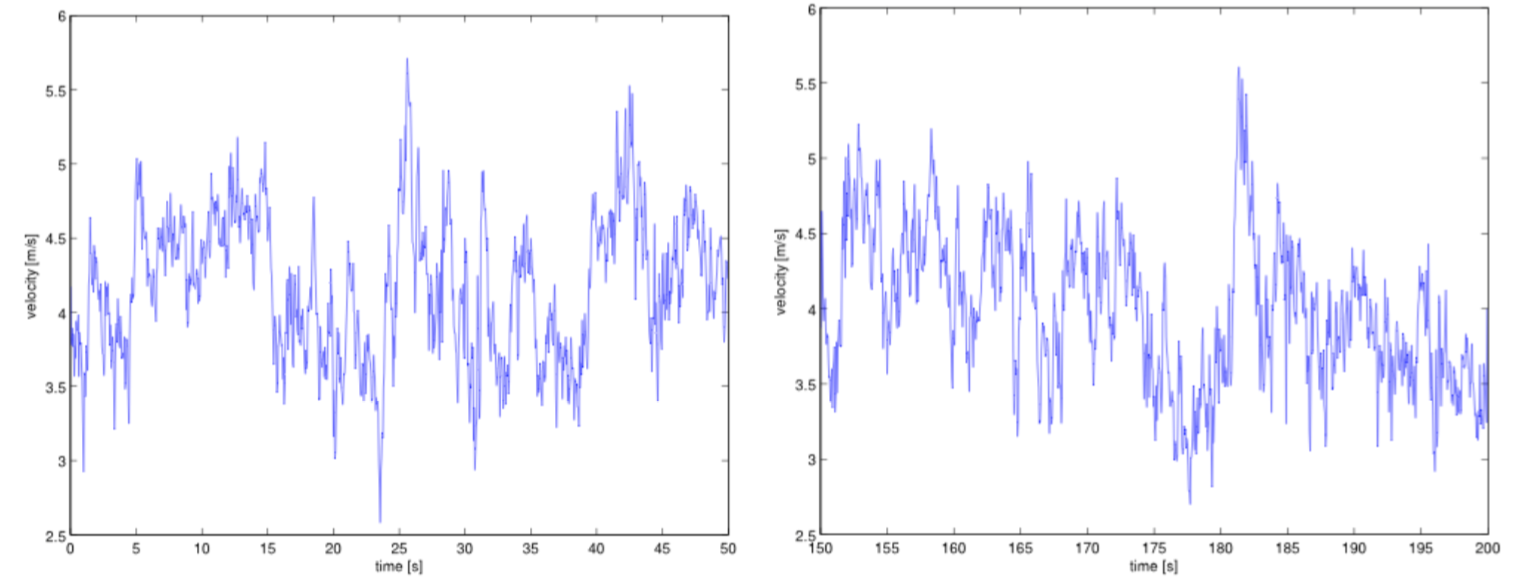
\includegraphics[width=0.8\textwidth]{timetrace1}
  	\end{figure}
  	\item Since $U$ is a random variable, its value is unpredictable for a turbulent flow.
  	\item Thus, any theory used to predict a particular value for $U$ will likely fail.
  	\item As we saw, however, certain statistical measures (histogram) appear to be reproducible. 
  \end{itemize}
\end{frame}

%------------------------------------------------
\begin{frame}{Basic Properties of Turbulence}
\begin{itemize}
  	\item Consider the velocity field $U$.
  	\begin{figure}
  		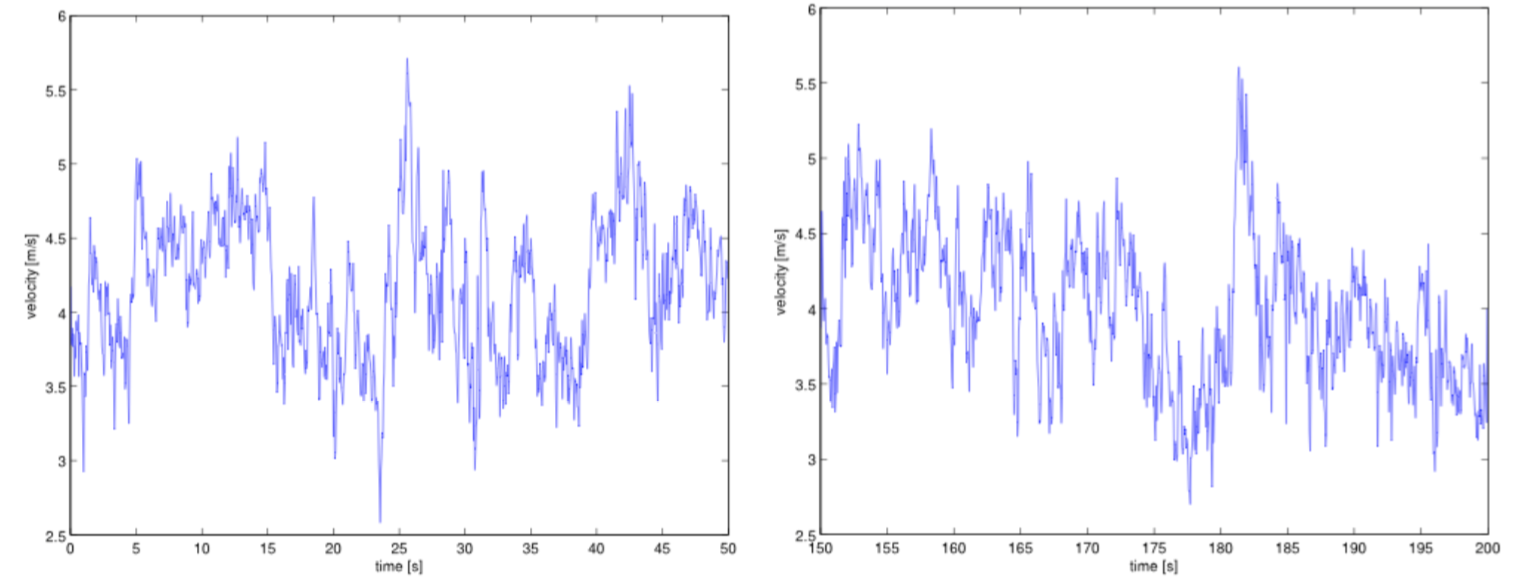
\includegraphics[width=0.8\textwidth]{timetrace1}
  	\end{figure}
  	\item In this time trace, notice that velocity is bounded, so there is some defined measure of turbulence intensity.
  	\item The ability to pick a mean value means that the flow field is not entirely random.
  	\item The time trace shows the existence of multiple time scales, which suggests that there are spatial features of different sizes and durations (i.e. a spectrum)
  \end{itemize}
\end{frame}
%------------------------------------------------
\subsection{Turbulence Spectrum}
%------------------------------------------------
\begin{frame}{Turbulence Spectrum}
\begin{itemize}
  	\item Example spectrum of wind speed near the ground
  	\begin{figure}
  		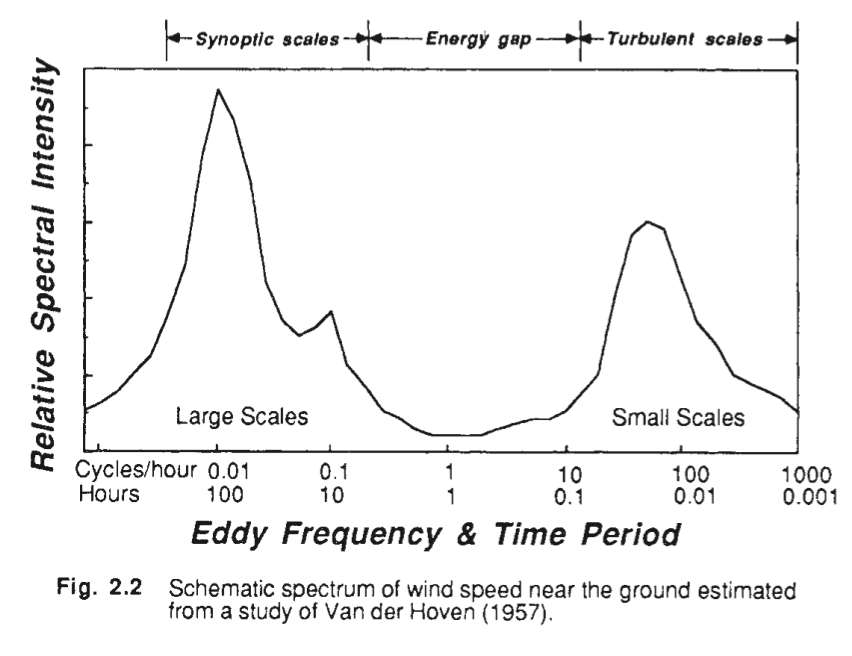
\includegraphics[width=0.8\textwidth]{spectrum}
  	\end{figure}
  	\centering \tiny{From Stull (1988)} 
  \end{itemize}
\end{frame}
%------------------------------------------------
\begin{frame}{Turbulence Spectrum}
\begin{itemize}
  	\item In the example spectrum, the vertical axis gives the contribution to the total turbulence energy by a particular eddy size, while the horizontal axis gives the size of eddies contained in the spectrum in terms of their duration.
  	\item Peaks show scales with the largest contribution.
  	\item The left peak, associated with a period of 100 hours, is associated with wind speed variations caused by frontal passages and weather systems.
  	\item The next peak is at 24 hours, which highlights the diurnal variations in wind speed.
  	\item The right peak, located between 10 seconds and 10 minutes, is evidence of small-scale eddies associated with turbulence.
  \end{itemize}
\end{frame}
%------------------------------------------------
\begin{frame}{Turbulence Spectrum}

\textbf{Spectral Gap}
\begin{itemize}
  	\item The relative lack of variation between the synoptic and microscale peaks is called the spectral gap.
  	\item Motions to the left are considered the \textit{mean flow}, and motions to the right are considered the \textit{turbulent flow}.
  	\item The spectral gap allows us to separate the flow into turbulent and non-turbulent parts.
  \end{itemize}
\end{frame}
%------------------------------------------------
\begin{frame}{Turbulence Spectrum}

\textbf{Mean and fluctuating parts}
\begin{itemize}
  	\item To isolate large scales from small scales, we can average over a period of 30 minutes to 1 hour
  	\item This allows us to average out the positive and negative fluctuations about the mean
  	\item The mean ($\overline{U}$; more later) is subtracted from the instantaneous value ($U$) to obtain the turbulent part
  	$$u^\prime = U - \overline{U}$$
  \end{itemize}
\end{frame}
%------------------------------------------------
\begin{frame}{Turbulence Spectrum}

\textbf{Mean and fluctuating parts}
\begin{itemize}
  	\item You can think of the turbulent fluctuation $u^\prime$ as a gust of wind associated with variations lasting longer than an hour, while the mean wind $\overline{U}$ is the part of the wind with variations that last longer than an hour (or so).
  	\begin{figure}
  		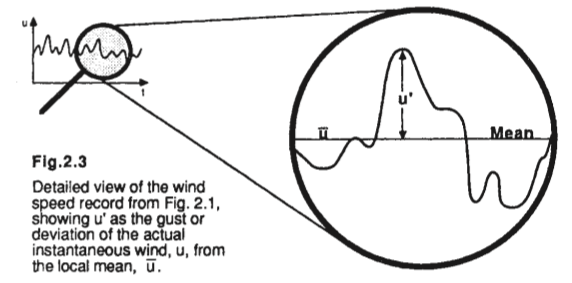
\includegraphics[width=0.8\textwidth]{turb1.png}
  	\end{figure}
  	\centering \tiny{From Stull (1988)} 
  	\item This underscores the need to describe turbulence statistically.
  \end{itemize}
\end{frame}


%------------------------------------------------
\subsection{Sample Space, CDF, and PDF}
\begin{frame}{Sample Space}
\begin{itemize}
  	\item In reality, a velocity field $U(\vec{x},t)$ is more complicated than a single random variable.
  	\item We need a wide range of statistical tools to characterize random variables.
  	\item In order to consider more general events, we need to think in terms of \textit{sample space}.
  	\item Consider an independent velocity variable $V$, which is the sample-space variable for $U$.
  \end{itemize}
\end{frame}

%------------------------------------------------

\begin{frame}{Sample Space}
  \begin{figure}[H]
  \centering
  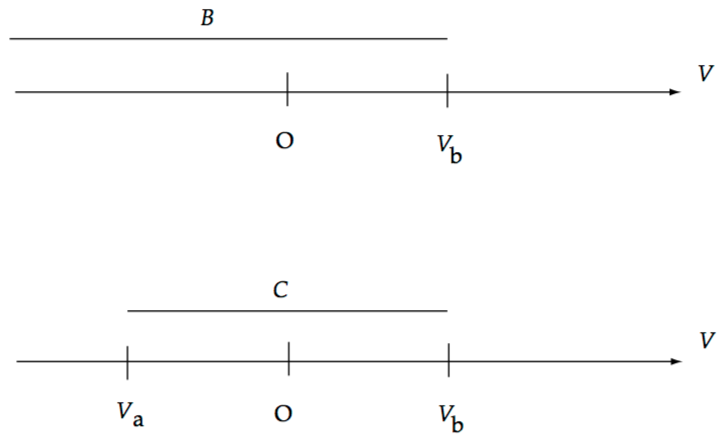
\includegraphics[width=0.65\textwidth]{samplespace.png}
  \end{figure}
  \begin{align*}
  B &\equiv \{U < V_b \}\\C &\equiv \{V_a \leq U < V_b \}
  \end{align*}
  $B$ and $C$ are events (or values) that correspond to different regions of the sample space (\textit{i.e.}, velocity field).
  
\end{frame}

%------------------------------------------------

\begin{frame}{Probability}
\begin{itemize}
  	\item Using the previous example, the probability of event $B$ is given as:
  	$$p=P(B)=P\{U<V_b\}$$
  	\item This is the likelihood of $B$ occurring ($U<V_b$).
  	\item $p$ is a real number, $0 \leq p \leq 1$.
  	\item $p = 0$ is an impossible event.
  	\item $p = 1$ is a certain event.
  \end{itemize}
\end{frame}

%------------------------------------------------

\begin{frame}{Cumulative Distribution Function}
\begin{itemize}
  	\item The probability of any event is determined by the cumulative distribution function (CDF)
  	$$F(V) \equiv P\{U<V\}$$
  	\item For event $B$:
  	$$P(B) = \{U < V_b \} = F(V_b)$$
  	\item For event $C$:
  	\begin{align*}
  	P(C) &= \{V_a \leq U < V_b \} = P\{U < V_b \} - P\{U < V_a \}\\ &= F(V_b) - F(V_a)
  	\end{align*}
  \end{itemize}
\end{frame}

%------------------------------------------------

\begin{frame}{Cumulative Distribution Function}
Three basic properties of CDF:
\begin{itemize}
  	\item $F(-\infty) = 0$, since $\{U < -\infty\}$ is impossible.
  	\item $F(\infty) = 1$, since $\{U > \infty\}$ is impossible.
  	\item $F(V_b) \geq F(V_a)$, for $V_b > V_a$, since $p > 0$. Thus, $F$ is a non-decreasing function.  
  \end{itemize}
\end{frame}

%------------------------------------------------

\begin{frame}{Probability Density Function}
The probability density function (PDF) is the derivative of the CDF
$$f(V)\equiv \frac{d F(v)}{dV}$$
Based on the properties of the CDF, it follows that:
\begin{itemize}
  	\item $f(V) \geq 0$
  	\item $\int^{\infty}_{-\infty} f(V) dV = 1$
  	\item $f(-\infty) = f(\infty) = 0$
  \end{itemize}
\end{frame}

%------------------------------------------------

\begin{frame}{Probability Density Function}

The probability that a random variable is contained within a specific interval is the integral of the PDF over that interval 
\begin{align*}
P(C) = P\{V_a \leq U < V_b \} &= F(V_b) - F(V_a)\\
&= \int^{V_b}_{V_a} f(V) dV
\end{align*}

Or, for a very small interval $dV_s$:
\begin{align*}
P(C_s) = P\{V_a \leq U < V_a + dV_s \} &= F(V_a + dV_s) - F(V_a)\\
&= f(V_a)dV_s
\end{align*}

\end{frame}

%------------------------------------------------

\begin{frame}{Probability Density Function}
More details about the PDF $f(V)$:
\begin{itemize}
	\item $f(V)$ is the probability per unit distance in the sample space -- hence, the term \textit{density}.
	\item $f(V)$ has dimensions of $U^{-1}$, while the CDF is dimensionless.
	\item The PDF fully characterizes the statistics of a signal (random variable).
	\item If two or more signals have the same PDF, then they are considered to be statistically identical.
	\end{itemize}
\end{frame}

%------------------------------------------------

\begin{frame}{CDF (top) vs. PDF (bottom)}
  \begin{figure}[H]
  \centering
  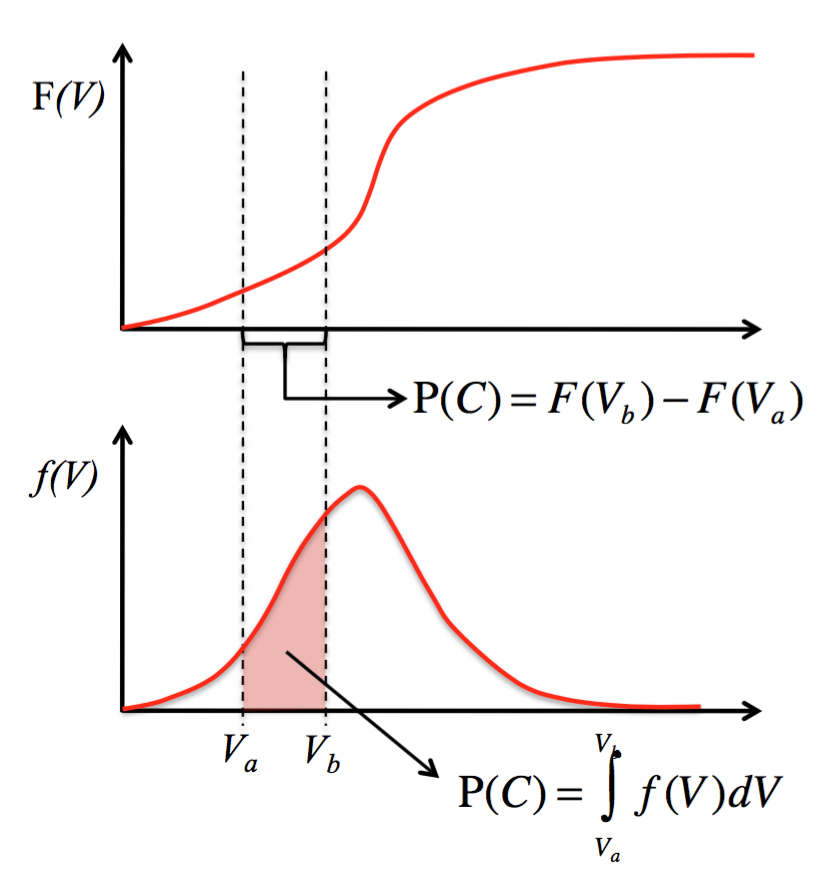
\includegraphics[width=0.7\textwidth]{cdfpdf.png}
  \end{figure}
\end{frame}

%------------------------------------------------
\subsection{The Mean}
\begin{frame}{The Mean}
We can also define a signal by its individual statistics, which collectively describe the PDF.
~\\~\\
The mean (or expected) value of a random variable $U$ is given by:
$$\overline{U} \equiv \int^{\infty}_{-\infty} Vf(V)dV$$
or in discrete form:
$$\overline{U} \equiv \frac{1}{N} \sum^N_{i=1} V_i$$
The mean represents the probability-weighted sum of all possible values of $U$.
\end{frame}
%------------------------------------------------

\begin{frame}{The Mean: Temporal Averaging}

\begin{itemize}
	\item For a continuous function at point in space $s=(x,y,z)$ over a time period $P$, where the turbulence is assumed to be \textit{stationary} (the statistics are \textbf{NOT} changing over the averaging period), the time average is given by: $$\overline{u}^t(s) = \frac{1}{P} \int^{t=t_0+P}_{t=t_0} u(t,s) dt$$
	\item For discrete data uniformly spaced in time, where $P=N\Delta t$: $$\overline{u}^t(s)=\frac{1}{N} \sum^{N}_{i=1} u(t,s)$$
\end{itemize}

\end{frame}

%------------------------------------------------

\begin{frame}{The Mean: Spatial Averaging}

\begin{itemize}
	\item Applies at in instant in time and is given as an integral of the spatial domain $S$:
	$$\overline{u}^s(t) = \frac{1}{S} \int_{S} u(t,s) dS$$
	\item Over some volume $S=\Delta x \Delta y \Delta z$:
	$$\overline{u}^s(t) = \frac{1}{\Delta x \Delta y \Delta z} \int \int_{S} \int u(t,x,y,z) dx dy dz$$
	\item For line averaging uniformly spaced data in space, where $Y=N\Delta y$:
	$$\overline{u}^s(t) = \frac{1}{Y} \int^{y=Y}_{y=0} u(t,s) dy$$
	or discretely
	$$\overline{u}^s(t) = \frac{1}{Y}\sum^{N}_{i=1} u(t,s)$$
\end{itemize}

\end{frame}

%------------------------------------------------

\begin{frame}{The Mean: Ensemble Averaging}

\begin{itemize}
	\item Averaging over a number ($N$) of experiments at a point in space. This method of averaging tends to minimize random experimental errors by repeating an experiment.
	$$\overline{u}^e(t,s) = \frac{1}{N}\sum^{N}_{i=1} u_i(t,s)$$
\end{itemize}
\end{frame}

%------------------------------------------------

\begin{frame}{The Mean: Ergodicity}

\begin{itemize}
	\item If the turbulence is both \textit{homogeneous} and \textit{stationary}, the time, space, and ensemble averages should be the same, namely
	$$\overline{u}^t=\overline{u}^s=\overline{u}^e=\overline{u}$$
	\item homogeneous turbulence $\Rightarrow$ statistics are invariant of coordinate translation
	\item stationary turbulence, $\Rightarrow$ the statistics are invariant to the choice of time window
	\item In the atmosphere there are many occasions when turbulence is neither homogeneous (e.g., around trees or buildings) or stationary (e.g., evening decay of the CBL)
	\item We must be very careful in applying the various types of averaging.
\end{itemize}
\end{frame}

%------------------------------------------------

\begin{frame}{The Mean: Ergodicity}

\begin{itemize}
	\item Consider this time series of potential temperature during the evening transition. These data clearly show the diurnal decrease of temperature in evening.  
	\item If we choose an averaging time of 1 hr, we will be including this diurnal variation in our fluctuations. 
	\item This problem may be avoided by using smaller averaging times or using linear detrending techniques
	\begin{figure}
		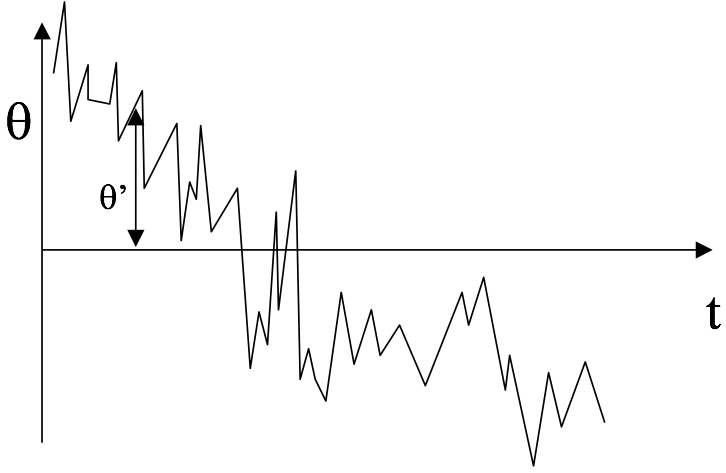
\includegraphics[width=0.5\textwidth]{nonstationary.png}
	\end{figure}
\end{itemize}
\end{frame}

%------------------------------------------------
\subsection{Reynolds Averaging}
\begin{frame}{Reynolds Averaging}

\begin{itemize}
	\item We saw that the spectral gap allows the separation of a flow field into mean and perturbation parts.
	\item The formal procedure of applying this separation is called \textbf{Reynolds decomposition} or \textbf{Reynolds averaging}.
	\item Accordingly, it is important to discuss the properties of the mean in this context.
	\item We will use this procedure and rules when deriving the turbulence equations (next lecture).
\end{itemize}
\end{frame}
%------------------------------------------------
\begin{frame}{Reynolds Averaging}

\textbf{Rules of averaging:}
\begin{itemize}
	\item $\overline{c} = c$, where $c$ is a constant
	\item $\overline{(c\; A)} = c\; \overline{A}$
	\item $\overline{(\overline{A})} = \overline{A}$
	\item $\overline{(\overline{A}\;B)} = \overline{A}\; \overline{B}$
	\item $\overline{(A+B)} = \overline{A} + \overline{B}$
	\item $\overline{\left(\cfrac{dA}{dt}\right)} = \cfrac{d\overline{A}}{dt}$
\end{itemize}
\end{frame}
%------------------------------------------------
\begin{frame}{Reynolds Averaging}

\begin{itemize}
	\item Let's apply these rules to variables that have been split into their mean and perturbation parts.
	\item Let $A = \overline{A} + a^\prime$ and $B = \overline{B} + b^\prime$
	\item Start with $A$
	$$\overline{(A)} = \overline{(\overline{A} + a^\prime)} = \overline{(\overline{A})} + \overline{a^\prime} = \overline{A} + \overline{a^\prime}$$
	The only way this is true is if $\overline{a^\prime} = 0$, which makes sense if we consider the definition of the mean (i.e., the sum of positive perturbations from the mean equals the sum of the negative perturbations).
\end{itemize}
\end{frame}
%------------------------------------------------
\begin{frame}{Reynolds Averaging}

\begin{itemize}
	\item Consider another example:
	$$\overline{(\overline{B}\;a^\prime)} = \overline{B}\; \overline{a^\prime} = \overline{B}\cdot 0 = 0$$
	\item Similarly, $\overline{(\overline{A}\;b^\prime)} = 0$
	\item Lastly:
	\begin{align*}
	\overline{A\; B} &= \overline{(A + a^\prime)(B+ b^\prime)} = \overline{\overline{A}\; \overline{B} + \overline{A}\; b^\prime + a^\prime\; \overline{B} + a^\prime\; b^\prime}\\
	& = \overline{\overline{A}\; \overline{B}} + \underbrace{\overline{\overline{A}\; b^\prime}}_{=0} + \underbrace{\overline{\overline{B}\; a^\prime}}_{=0} + \overline{a^\prime\; b^\prime}\\
	&= \overline{A}\;\overline{B} + \overline{a^\prime\; b^\prime}
	\end{align*}
	Where $\overline{a^\prime\; b^\prime}$ is covariance (more later), or variance if $a^\prime = b^\prime$. 
	
	Note: although $\overline{a^\prime}=0$ and $\overline{b^\prime}=0$, $\overline{a^\prime\; b^\prime}$ is \textbf{not} necessarily 0.
\end{itemize}
\end{frame}

%------------------------------------------------
\subsection{Moments}
\begin{frame}{Variance}

Recall that a \textit{fluctuation} (or perturbation) from the mean:
$$u^\prime \equiv U - \overline{U}$$
The \textit{variance} is just the mean-square fluctuation:
\begin{align*}
\sigma_u^2 = \text{var}(U) &= \overline{{u^\prime}^2}\\
&= \int^{\infty}_{-\infty} (V - \overline{U})^2 f(V) dV 
\end{align*}
Or, in discrete form:
$$\sigma_u^2 = \frac{1}{N-1^*} \sum^N_{i=1} (V_i - \overline{U})^2$$

Variance essentially measures how far a set of (random) numbers are spread out from their mean.
\newline\newline
\scriptsize{$^*$note the ($N-1$). This is the \href{https://en.wikipedia.org/wiki/Bessel\%27s_correction}{\color{UUcrimson}\underline{Bessel correction}} -- used to correct for bias.}

\end{frame}

%------------------------------------------------

\begin{frame}{Standard Deviation}

The \textit{standard deviation}, or root-mean square (rms) deviation, is just the square-root of the variance:
$$\sigma_u \equiv \text{sdev}(U) = \sqrt{\sigma_u^2} = \sqrt{\overline{{u^\prime}^2}}$$

The standard deviation basically measures the amount of variation of a set of numbers.
\end{frame}

%------------------------------------------------

\begin{frame}{Other moments}

The $n^{th}$ central moment is defined as:
$$\mu_n \equiv \overline{{u^\prime}^n} = \int^{\infty}_{-\infty} (V - \overline{U})^n f(V)dV$$
\end{frame}

%------------------------------------------------

\begin{frame}{Standardized Moments}

It is often advantageous to express variables as standardized random variables. These standardized variables have zero mean and unit variance.\newline\newline
The standardized version of $U$ (centered and scaled) is given by:
$$\hat U \equiv \frac{U - \overline{U}}{\sigma_u}$$
Accordingly, the $n^{th}$ standardized moments are expressed as:
$$\hat \mu_n \equiv \frac{\overline{{u^\prime}^n}}{\sigma_u^n} = \frac{\mu_n}{\sigma_u^n}  = \int^{\infty}_{-\infty} \hat V^n \hat f(\hat V)d \hat V$$

\end{frame}

%------------------------------------------------

\begin{frame}{Other moments}

Different moments each describe an aspect of the shape of the PDF:
\begin{itemize}
	\item $\mu_1$      = mean (expected value)
	\item $\mu_2$      = variance (spread from the mean)
	\item $\hat \mu_3$ = skewness (asymmetry of PDF)
	\item $\hat \mu_4$ = kurtosis (sharpness of the PDF peak)
\end{itemize}

\end{frame}

%------------------------------------------------

\begin{frame}{Example PDFs}

Read Pope (Chapter 3.3) for descriptions of different PDFs. \newline\newline Examples include:
\begin{itemize}
	\item uniform
	\item exponential
	\item Gaussian
	\item log-normal
	\item gamma
	\item Delta-function
	\item Cauchy
\end{itemize}

\end{frame}

%------------------------------------------------
\subsection{Joint Random Variables}
\begin{frame}{Joint Random Variables}

So far, our statistical description has been limited to single random variables. However, turbulence is governed by the Navier-Stokes equations, which are a set of 3 coupled PDEs.\newline\newline
We expect this will result in some correlation between different velocity components.

\end{frame}

%------------------------------------------------

\begin{frame}{Joint Random Variables}
  Example: turbulence data from the ABL: scatter plot of horizontal (u) and vertical (w) velocity fluctuations.
  \begin{figure}[H]
  \centering
  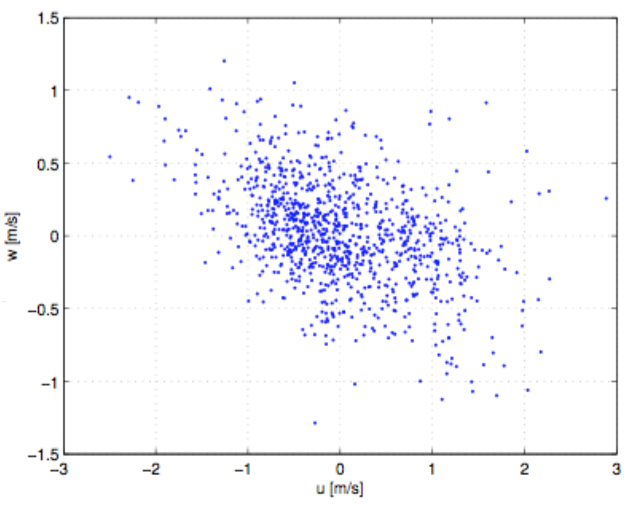
\includegraphics[width=0.7\textwidth]{jr1.png}
  \end{figure}
  The plot appears to have a pattern (\textit{i.e.}, negative slope).
\end{frame}

%------------------------------------------------

\begin{frame}{Joint Random Variables - Sample Space}
  We will now extend the previous results from a single velocity component to two or more.\newline\newline
  The sample-space variables corresponding to the random variables $U=\{U_1,U_2,U_3\}$ are given by $V=\{V_1,V_2,V_3\}$.
\end{frame}

%------------------------------------------------

\begin{frame}{Joint Random Variables - CDF}
  
  \setlength{\fboxsep}{0pt}
\setlength{\fboxrule}{1pt}
\begin{columns}[T]
    \begin{column}{.55\textwidth}
    \begin{minipage}[c][.6\textheight][c]{\linewidth}
    The joint CDF (jCDF) of the random variables ($U_1, U_2$) is given by:
  $$F_{12}(V_1,V_2) \equiv P\{U_1 < V_1, U_2 < V_2\}$$
  This is the probability of the point ($V_1,V_2$) lying inside the shaded region 
      \end{minipage}
    \end{column}
    \begin{column}{.55\textwidth}
      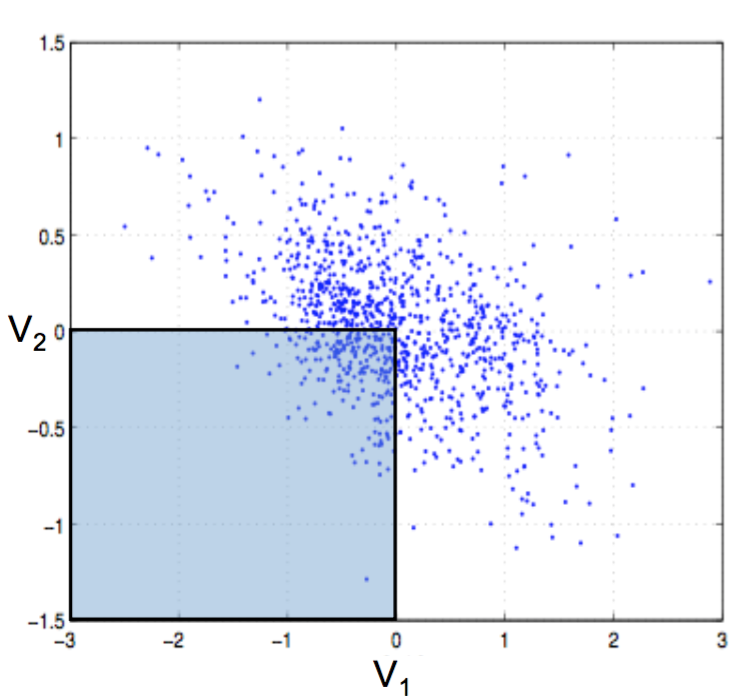
\includegraphics[width=\textwidth]{jr2.png}
    \end{column}
  \end{columns}
  
\end{frame}

%------------------------------------------------

\begin{frame}{Joint Random Variables - CDF}
  The jCDF has the following properties:
  
  \begin{itemize}
  	\item $F_{12}(V_1 + \delta V_1, V_2 + \delta V_2) \geq F_{12}(V_1, V_2)$ (non-decreasing) \newline for all $\delta V_1\geq0$, $\delta V_2\geq0$\newline
  	\item $F_{12}(-\infty,V_2) = P\{U_1<-\infty,U_2<V_2\} = 0$\newline since $\{U_1 < -\infty\}$ is impossible.\newline
  	\item $F_{12}(\infty,V_2) = P\{U_1<\infty,U_2<V_2\} = P\{U_2<V_2\}\newline F_{12}(\infty,V_2) = F_2(V_2)$, since $\{U_1 < \infty\}$ is certain.\newline
  \end{itemize}

  In the last example, $F_2(V_2)$ is called the \textit{marginal CDF}.
\end{frame}

%------------------------------------------------

\begin{frame}{Joint Random Variables - PDF}
  The joint PDF (jPDF) is defined as:
  $$f_{12}(V_1, V_2) \equiv \frac{\partial^2}{\partial V_1 \partial V_2}F_{12}(V_1,V_2)$$
  If we integrate over $V_1$ and $V_2$, we get the probability:
  $$P\{V_{1a} \leq U_1 < V_{1b}, V_{2a} \leq U_2 < V_{2b}\} = \int^{V_1b}_{V_1a} \int^{V_2b}_{V_2a} f_{12}(V_1,V_2)dV_2dV_1$$
  
\end{frame}

%------------------------------------------------

\begin{frame}{Joint Random Variables - PDF}
  Based on the jCDF, the jPDF has the following properties:
  \begin{itemize}
  	\item $f_{12} (V_1,V_2) \geq 0$\newline
  	\item $\int^{\infty}_{-\infty} f_{12}(V_1,V_2)dV_1 = f_2(V_2)$\newline
  	\item $\int^{\infty}_{-\infty} \int^{\infty}_{-\infty} f_{12}(V_1,V_2)dV_1dV_2 = 1$\newline
  \end{itemize}
  
  In the middle example, $f_2(V_2)$ is called the \textit{marginal PDF}. Practically speaking, we find the PDF of a time (or space) series by:
  \begin{itemize}
  	\item Create a histogram of the series(group values into bins)
  	\item Normalize the bin weights by the total \# of points
  \end{itemize}
\end{frame}

%------------------------------------------------

\begin{frame}{Joint Random Variables - Means}
  
  Similar to the single variable form, if we have $Q(U_1,U_2)$:
  $$\overline{Q(U_1,U_2)} \equiv \int^{\infty}_{-\infty} \int^{\infty}_{-\infty} Q(V_1,V_2)f_{12}dV_2dV_1$$
  We can use this equation to define a few important statistics.
  
\end{frame}

%------------------------------------------------

\begin{frame}{Joint Random Variables - Covariance}
  We can define \textit{covariance} as:
  \begin{align*}
  \text{cov}(U_1,U_2) &\equiv \newline \overline{u_1^\prime u_2^\prime} \\ &= \int^{\infty}_{-\infty} \int^{\infty}_{-\infty}(V_1 - \overline{U_1})(V_2 - \overline{U_2}) f_{12}(V_1,V_2)dV_2dV_1
  \end{align*}
  Or for discrete data
  \begin{align*}
  \text{cov}(U_1,U_2) &\equiv \overline{u_1^\prime u_2^\prime} \\ &= \frac{1}{N-1} \sum^N_{j-1} (V_{1j} - \overline{U_1})(V_{2j} - \overline{U_2})
  \end{align*}
  Covariance is basically a measure of how much two random variables change together.
\end{frame}

%------------------------------------------------

\begin{frame}{Joint Random Variables - Covariance}
  Example: cov($w$,$\theta$) = $\overline{w^\prime \theta^\prime}$. This is the eddy flux concept.
  \begin{figure}
  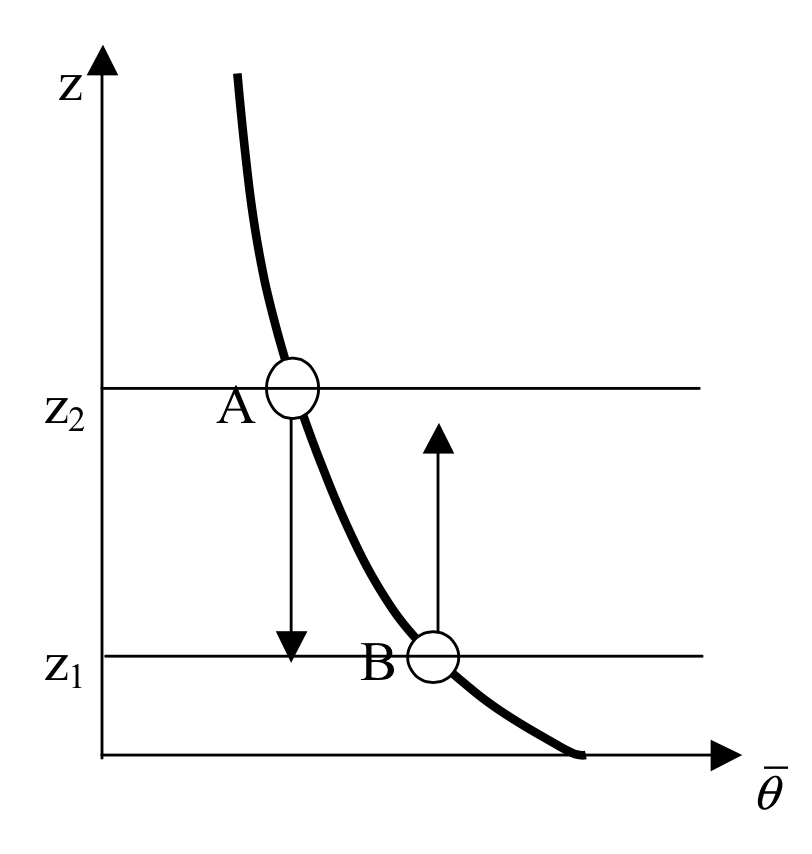
\includegraphics[width=0.47\textwidth]{flux.png}	
  \end{figure}
  Under convective conditions
	\begin{itemize}
		\item Parcel A: $w^{'} < 0$ and $\theta^{'} < 0 \rightarrow \overline{w^{'}\theta^{'}} > 0$ (positive heat flux)
		\item Parcel B: $w^{'} > 0$ and $\theta^{'} > 0 \rightarrow \overline{w^{'}\theta^{'}} > 0$ (positive heat flux)
	\end{itemize}
\end{frame}

%------------------------------------------------

\begin{frame}{Joint Random Variables - Correlation Coefficient}
  
  The \textit{correlation coefficient} is given by:
  $$\rho_{12} \equiv \frac{\overline{u_1^\prime u_2^\prime}}{\sqrt{\overline{{u_1^\prime}^2}\; \overline{{u_2^\prime}^2}}}$$
  Correlation coefficient has the following properties:
  \begin{itemize}
  	\item $-1 \leq \rho_{12} \leq 1$
  	\item Positive values indicate correlation.
  	\item Negative values indicate anti-correlation.
  	\item $\rho_{12} = 1$ is perfect correlation.
  	\item $\rho_{12} = -1$ is perfect anti-correlation.
  \end{itemize}
\end{frame}

%------------------------------------------------
\subsection{Two-point Statistical Measures}
\begin{frame}{Two-point Statistical Measures}
  
  \textit{Autocovariance} measures how a variable changes with different lags, $s$.
  $$R(s) \equiv \overline{u(t) u(t+s)}$$
  or the \textit{autocorrelation function}
  $$\rho(s) \equiv \frac{ \overline{u(t)u(t+s)}}{u(t)^2}$$
  Or for the discrete form
  $$\rho(s_j) \equiv \frac{ \sum^{N-j-1}_{k=0}(u_ku_{k+j})}{\sum^{N-1}_{k=0}(u_k^2)}$$
  
\end{frame}

%------------------------------------------------

\begin{frame}{Two-point Statistical Measures}
  
  Notes on autocovariance and autocorrelation
  \begin{itemize}
  	\item These are very similar to the covariance and correlation coefficient
  	\item The difference is that we are now looking at the linear correlation of a signal with itself but at two different times (or spatial points), i.e. we lag the series.
  	\item We could also look at the cross correlations in the same manner (between two different variables with a lag).
  	\item $\rho(0) = 1$ and $|\rho(s)| \leq 1$
  \end{itemize}
  
\end{frame}
%------------------------------------------------

\begin{frame}{Two-point Statistical Measures}
  
\setlength{\fboxsep}{0pt}
\setlength{\fboxrule}{1pt}
\begin{columns}[T]
    \begin{column}{.45\textwidth}
    \begin{itemize}
    	\item In turbulent flows, we expect the correlation to diminish with increasing time (or
distance) between points
    	\item We can use this to define an integral time (or space) scale. It is defined as the time lag where the integral $\int \rho(s)ds$ converges. 
    	\item It can also be used to define the largest scales of motion (statistically).
    \end{itemize}
    \end{column}
    \begin{column}{.55\textwidth}
    \begin{minipage}[c][.6\textheight][c]{\linewidth}
      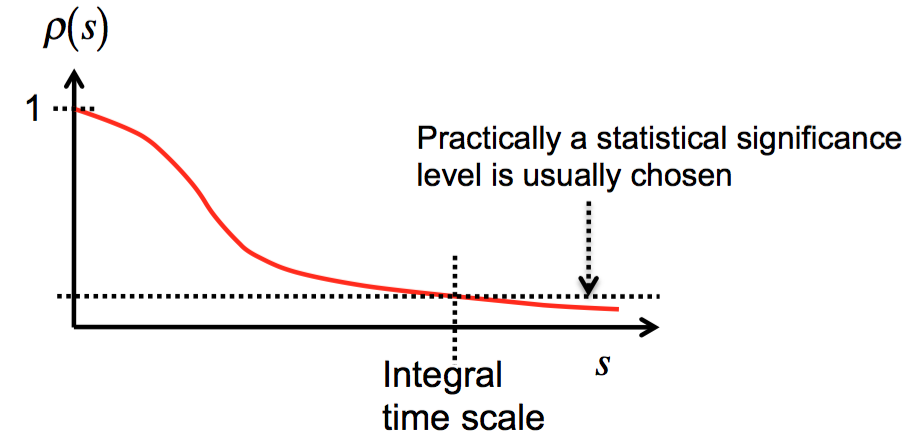
\includegraphics[width=\textwidth]{auto1.png}
      \end{minipage}
    \end{column}
  \end{columns}
  
\end{frame}

%------------------------------------------------

\begin{frame}{Two-point Statistical Measures}
  
  The \textit{structure function} is another important two-point statistic.
  $$D_n(r) \equiv \overline{[U_1(x+r,t) - U_1(x,t)]^n}$$
  \begin{itemize}
  	\item This gives us the average difference between two points separated by a distance $r$ raised to a power $n$.
  	\item In some sense it is a measure of the moments of the velocity increment PDF.
  	\item Note the difference between this and the autocorrelation which is statistical linear correlation (\textit{i.e.}, multiplication) of the two points.
  \end{itemize}
  
\end{frame}

%------------------------------------------------
\subsection{Taylor's Frozen Turbulence Hypothesis}
\begin{frame}{Taylor's Frozen Turbulence Hypothesis}

\begin{itemize}
	\item It is very difficult to produce highly spatially resolved measurements of temperatures and velocities over a large spatial region at one instant in time
	\item Thus, we sually measure over large time periods at very few points in space (i.e., a sonic anemometer mounted on a tower or a hot-wire probe in a wind tunnel). 
	\item G.I. Taylor (1938) proposed an idea that for some special cases, turbulence might be considered ``frozen'' as it advects pass our measuring device. 
\end{itemize}
\end{frame}

%------------------------------------------------

\begin{frame}{Taylor's Frozen Turbulence Hypothesis}

\begin{itemize}
	\item As a result turbulence measurements that are made as a function of time can be translated into a corresponding spatial measurement.
	\item  This hypothesis is useful for cases where turbulent eddies evolve with a timescale longer than the time scale it takes the eddy to be advected past the sensor.
\end{itemize}
\end{frame}

%------------------------------------------------

\begin{frame}{Taylor's Frozen Turbulence Hypothesis}
\begin{figure}
	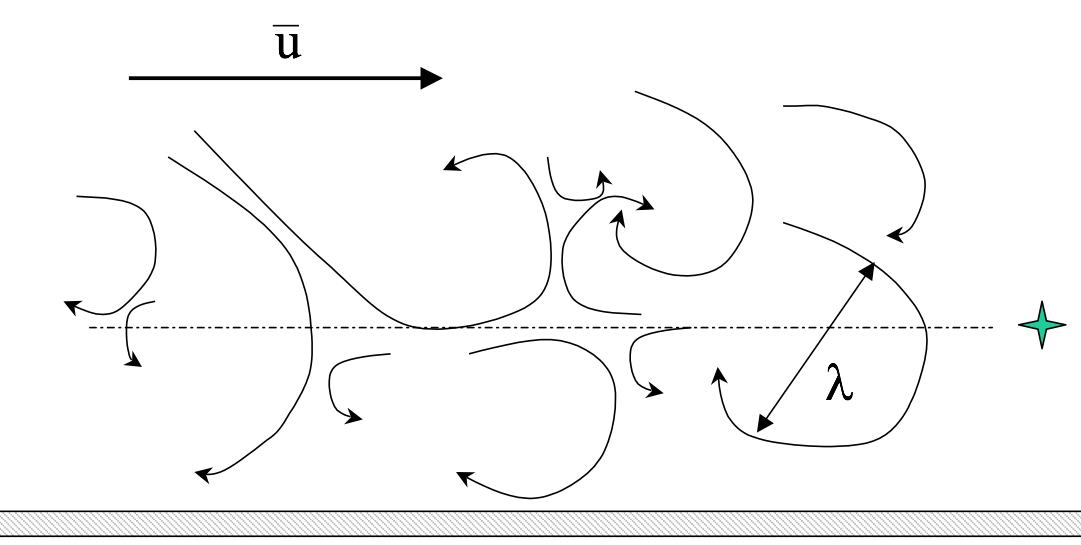
\includegraphics[width=0.6\textwidth]{frozen.png}
\end{figure}
\begin{itemize}
	\item Consider schematic of turbulence in a boundary layer. 
	\item One way to measure the velocities along the line shown at an instant in time, would be to place sensors all along the line.
\end{itemize}
\end{frame}

%------------------------------------------------

\begin{frame}{Taylor's Frozen Turbulence Hypothesis}
\begin{figure}
	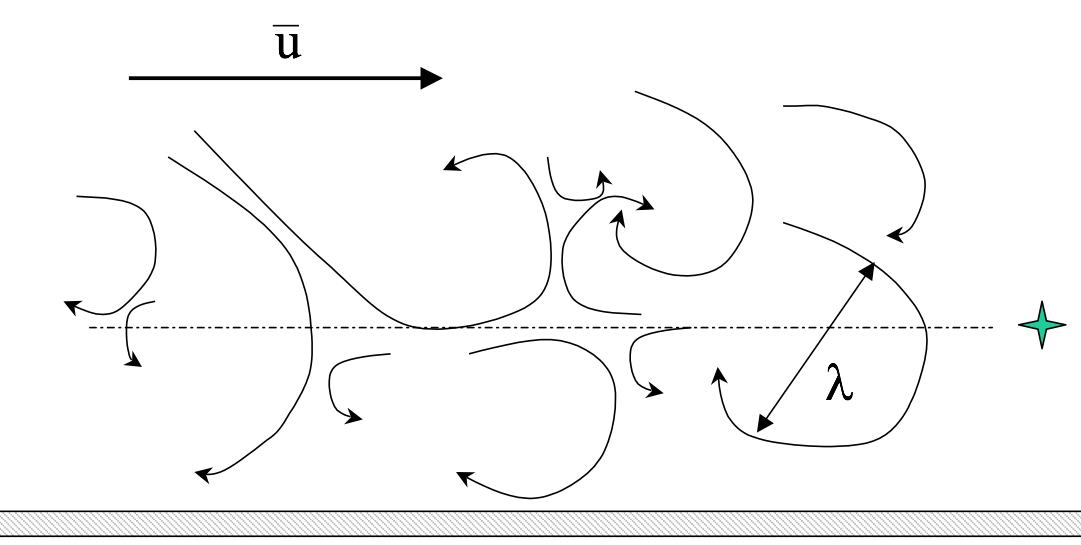
\includegraphics[width=0.6\textwidth]{frozen.png}
\end{figure}
\begin{itemize}
	\item Another way would be to move the probe very quickly through the flow at some known velocity assuming the flow doesn’t change much while you traverse it. 
	\item One other way would be to leave the probe in one place and allow the fluid to advect past the probe. 
	\item The last two ways utilize Taylor’s Frozen Turbulence hypothesis
\end{itemize}
\end{frame}

%------------------------------------------------

\begin{frame}{Taylor's Frozen Turbulence Hypothesis}

\begin{itemize}
	\item Following Stull (1988), the substantial derivative is zero for Taylor's Hypothesis
	\item Thus, $$\frac{\partial \zeta}{\partial t} = -\overline{u}\frac{\partial \zeta}{\partial x}-\overline{v}\frac{\partial \zeta}{\partial y}-\overline{w}\frac{\partial \zeta}{\partial z}$$
\end{itemize}
\end{frame}

%------------------------------------------------
\end{document}

